\documentclass[border=2pt]{standalone}
\usepackage{pgfplots, transparent}
\usetikzlibrary{arrows.meta}
\definecolor{blogred}{HTML}{ff6868}
\begin{document}
    \resizebox{10cm}{!} {
        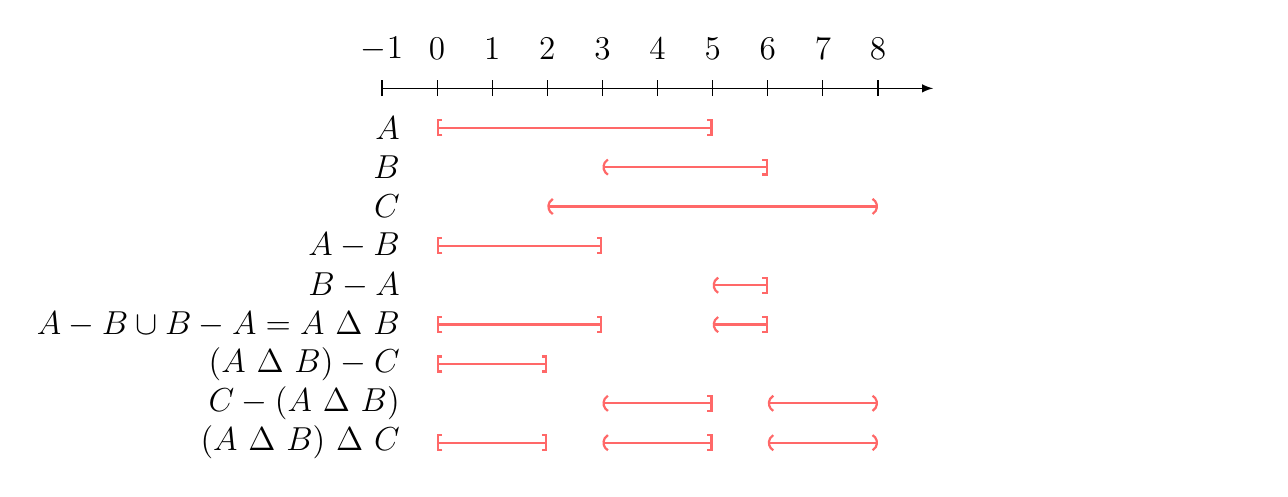
\begin{tikzpicture} [
            xscale = 0.7,
            yscale = -1
        ]
            \tikzset{basestyle/.style = {thick, blogred}}
            \tikzset{crange/.style    = {basestyle, Bracket-Bracket}}
            \tikzset{orange/.style    = {basestyle, Parenthesis-Parenthesis}}
            \tikzset{lorange/.style   = {basestyle, Parenthesis-Bracket}}
            \tikzset{rorange/.style   = {basestyle, Bracket-Parenthesis}}

            % x-axis specification
            \draw [-latex] (-1,0) -- (9,0);
            \foreach \x in {-1,0,1,...,8} {
                \draw (\x, 0.1) -- (\x,-0.1);
                \draw (\x,-0.5) node {\large $\x$};
            }

            \draw (-0.5,0.5) node [left] {\large $A$}; \draw [crange] (0,0.5) -- (5,0.5);

            \draw (-0.5,1.0) node [left] {\large $B$}; \draw [lorange] (3,1.0) -- (6,1.0);

            \draw (-0.5,1.5) node [left] {\large $C$}; \draw [orange] (2,1.5) -- (8,1.5);

            \draw (-0.5,2.0) node [left] {\large $A - B$}; \draw [crange] (0,2.0) -- (3,2.0);

            \draw (-0.5,2.5) node [left] {\large $B - A$}; \draw [lorange] (5,2.5) -- (6,2.5);

            \draw (-0.5,3.0) node [left] {\large $A - B \cup B - A = A \ \Delta \ B$};
            \draw [crange] (0,3.0) -- (3,3.0);
            \draw [lorange] (5,3.0) -- (6,3.0);
            \draw (8,3.0) node [right] {\large \phantom{$A - B \cup B - A = A \ \Delta \ B$}};

            \draw (-0.5,3.5) node [left] {\large $(A \ \Delta \ B) - C$};
            \draw [crange] (0,3.5) -- (2,3.5);

            \draw (-0.5,4.0) node [left] {\large $C - (A \ \Delta \ B)$};
            \draw [lorange] (3,4.0) -- (5,4.0);
            \draw [orange] (6,4.0) -- (8,4.0);

            \draw (-0.5,4.5) node [left] {\large $(A \ \Delta \ B) \ \Delta \ C$};
            \draw [crange] (0,4.5) -- (2,4.5);
            \draw [lorange] (3,4.5) -- (5,4.5);
            \draw [orange] (6,4.5) -- (8,4.5);
        \end{tikzpicture}
    }
\end{document}
